\documentclass{report}
\usepackage{graphicx}
\usepackage[numbers]{natbib}
\begin{document}

\title{The Prandtl Investigation Development Specification}
\author{Ni\"el Agenbag}

\maketitle

\begin{abstract}
The Prandtl investigation has the goal of determining whether or not it is possible to build a high performance tailless glider with good handling qualities using the Prandtl spanwise circulation distribution as opposed to an elliptical spanwise circulation distrubtion, but without the addtional assistance of stability augmentation systems.  In this context high performance relates to the glider performance required for a world championship winning glider.  This is the development specification.
\end{abstract}


\chapter{Development framework}

\section{Introduction}

This is the development specifcation for the Prandtl investigation.  The Prandtl investigation has the goal of determining whether or not it is possible to build a high performance tailless glider with good handling qualities using the Prandtl spanwise circulation distribution as opposed to an elliptical spanwise circulation distrubtion, but without the addtional assistance of stability augmentation systems.  In this context high performance relates to the glider performance required for a world championship winning glider.

The description of the Prandtl lift distribution as applied to tailless aircraft is presented in \cite{PrandtlBowers}.  The inspiration for the Prandtl investigation came from the organizers of the Prandtl investigation listening to the podcast in \cite{omegataupodcastPrandtl}.

Ludwig Prandtl postulated that the optimal circulation distribution for a given span was elliptical as shown in \cite{Prandtl1921}.  Later he reformulated the problem and derived the optimal spanwise circulation distribution for a given air vehicle mass (\cite{Prandtl1933}).  This bell-shaped circulation distribution potentially has lower drag compared to the elliptical distribution as well as better handling qualities when applied to a tailless aircraft.

This investigation will attempt to determine whether the Prandtl spanwise circulation distribution has satisfactory performance and handling quality criteria as applied to a tailless aircraft configuration.

\section{Prandtl wing philosophy}

It is assumed that the parasitic drag or $C_{D0}$ is kept low for a tailless concept because the absence of the empennage reduces drag compared to a an aircraft that has vertical and horizontal control and stability surfaces.

The Prandtl wing has some additional advantages above the low drag of the tailless concept that uses the elliptical circulation distribution.  The following information is from \cite{omegataupodcastPrandtl}.

The Prandtl lift distribution is the circulation distribution that has the minimum induced drag for a specific amount of structure or mass.  It has 11\% less drag and 22\% more span compared to an elliptical circulation distribution.  The slope at the centre span and at the tip is zero for the Prandtl distribution.  The downwash for the Prandtl distribution is not uniform or constant as is the case with the elliptical distribution.  There is upwash at the tip of the wing for the Prandtl distribution.

Adverse yaw is kept in check with Prandtl distribution.  There is induced thrust at the tip of the wing during a control surface deflection.  This causes proverse yaw and helps the aircraft execute automatically coordinated turns.  Only a small contribution to lift comes from the span at the at the control surfaces and therefore there is no loss in lift as a resut of control deflections.  With an elliptical lift distribution there is a major disturbance of the circulation distribution during control surface deflection, resulting in inefficiencies.  This will hopefully not be the case for the Prandtl distribution.  The control surfaces must be in the last 30\% of span in order for the Prandtl distribution not to be affected by control surface deflection.

No additional drag is present for turn coordination from a rudder control surface because turns are already coordinated. This implies more efficient turn performance which is important for competition gliding.

The position where the downwash changes to upwash is a function of sweep angle.  Therefore if the aircraft is yawing this position changes spanwise.  This causes artificial yaw damping and consequently a tailless aircraft with a Prandtl distribution does not have dutch roll problems or lack of yaw stiffness.

The $C_{D0}$ value is further reduced because a Prandtl style wing is claimed (\cite{PrandtlPatent}) to have less wetted area compared to a wing design with an elliptical circulation distribution thas has the same lift capacity.

The Prandtl circulation distribution is achieved with taper, airfoils varying spanwise and twist varying spanwise in a non-linear fashion.


\subsection{A note on trim}


The aft fuselage shape can be used for trim.  Alternatively wing sweep may be used as trim, but since this implies heavy and crack prone hinges this approach is not favoured.

Large sea birds don't have tails hence messy landings.  They don't need it because they seldom land.

Evolution leads to a tail empennage structure disappearing as part of the engineering design iterations.  If you design an aircraft with a Prandtl circulation distribution and a horizontal tail surface on an empennage which also includes a rudder, you soon abandon the rudder, because it is never used.  The tail pitch moment is so small that the tailboom is much reduced until it morphs into the fuselage, or completely disappears.


\section{Goals}

\subsection{Performance}

What is meant by performance. Moving baseline since aircraft technology continuously progresses, but 53 to 1 $\frac{L}{D}$ ratio with good handling qualities was a championship winning glider in 2017.  This is the benchmark for the start of the investigation.

Must be done on a full scale aircraft.  Note the high angle of attack difference from \cite{ModelFlightNASA}


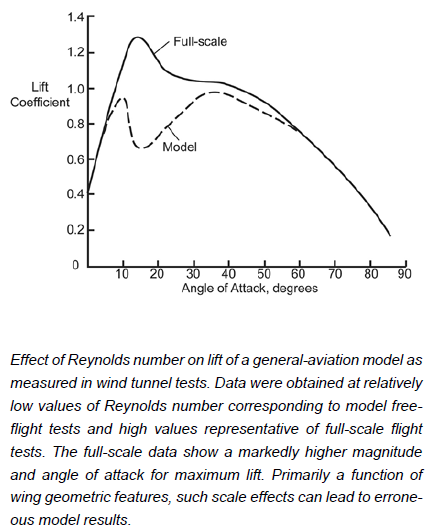
\includegraphics[width = 0.5\textwidth]{Pictures/ModelAeroVSFullSize.png}

\subsection{Handling qualities}

What is meant by handling qualities. Short period and phugoid. What it should be with references
MIL 8586
Cstar etc.

Also lateral handling qualities.

And pilot in the loop to verify using flight simulation.


\section{Cooper Harper Flying Qualities Rating Scale}\label{Sec:  CooperHarperMethodExplain}

\index{Handling qualities!Cooper Harper rating scale}

The Cooper Harper evaluation criterion \citep{CooperHarper} is a subjective method of evaluating aircraft handling qualities.  This is different from all the other evaluation methods presented in this study, since the other methods are mathematical/empirical in nature.  This method gives the pilot a way of having an influence on the design of the aircraft.  This is important since the pilot is the end user of the aircraft.

With this method, the pilot rates the aircraft controllability on a scale from 1 to 10, with 1 being the most favourable rating.  The Cooper Harper evaluation criterion is presented in Table \ref{tab:CooperHarper}.  

The Cooper Harper scale can only be used if an aircraft is available for flight testing or if an accurate flight simulator of the aircraft exists.  The flight simulator should be able to simulate pitching motion as well as normal (up and down) acceleration.  In addition to the hardware a group of pilots is also required in order to be able to conduct a handling qualities  study.  The pilot opinion of the aircraft is then obtained by letting the various pilots either test fly the aircraft or letting the pilots interact with the the simulator.  A questionnaire is then used to determine the Cooper Harper rating of the aircraft.

The Cooper Harper criterion will not be used in the gull-wing handling qualities study since neither a pitch flight simulator nor an aircraft were available for testing at the time of completion of this study.

\section{The Zacher Protocol}

\index{Handling qualities!Zacher protocol}

The Zacher Flight Test Protocol \citep{SailPlaneDesign} was developed by Hans Zacher specifically for sailplanes and uses flight tests and a questionnaire to evaluate the flying qualities of an aircraft.  This protocol was not applied to the gull-wing configuration since a prototype was not available for flight testing.

\section{Thumbprint Criterion Analysis}\label{sec: perfcriteria}

\index{Handling qualities!Thumbprint criterion}

The handling quality criterion presented here is based on the research presented in \cite{OHara}.  An application of the thumbprint criterion can be found in \verw{Wigartikel}{17}.
The method is based on the natural frequency and damping ratio of the aircraft dynamic modes.  

The criterion is summarised in the graph presented in Figure \ref{fig: shortperiodopinion}.  This graph is also known as the `thumbprint'.  An aircraft has satisfactory handling qualities when its short period damping ratio and natural frequency can be plotted in the centre of the contours of the `thumbprint' graph.  

\begin{figure}[htb]
	\begin{center}
		\includegraphics[width = 0.7\textwidth]{vingerafdruk.pdf}
	\end{center}

	\caption{Typical pilot opinion contours for the short period mode \citep{OHara}.}
	\label{fig: shortperiodopinion}
\end{figure}

\nomenclature[Rd -g noprefix]{$PR$}{Pilot rating (of aircraft handling qualities)}

The pilot opinion contours shown in the `thumbprint' (Figure \ref{fig: shortperiodopinion}) were constructed from flight tests.  Pilots were used to evaluate the handling qualities of so-called `variable stability' aircraft such as the USAF/CAL \mbox{T-33} \index{USAF/CAL \mbox{T-33}} aircraft.  The damping ratio and natural frequencies of a variable stability aircraft can be varied by adjusting the $CG$ of the aircraft.  Pilot opinions of several $CG$ configurations were compiled in the form of Figure \ref{fig: shortperiodopinion}.  The pilot opinions of the different configurations were expressed in pilot ratings ($PR$). \index{Pilot rating}  The pilot ratings correspond to the Cooper-Harper scale.  The thumbprint criterion requires two assumptions:

\begin{itemize}
	\item{The predominant variable sensed by the pilot is normal acceleration, as opposed to pitching acceleration.}
	\item{The short period response may be represented by that of a linear second order system.}
\end{itemize}

The thumbprint criterion is important for aircraft that do not have stability augmentation systems.  A linear second order system might not be able to approximate the dynamics of an aircraft that is stability augmented.

In order to use the thumbprint criterion, it is necessary to know the natural frequency and the damping ratio of the short period mode of an aircraft.  These values may be determined by means of the following methods:

\begin{itemize} 
	\item{Flight testing can be used to excite the short period aircraft mode independently of the phugoid mode.  The damping ratio and natural frequency can then be established by means of curve fitting techniques from flight test data.}
	\item{A mathematical model can be created that describes the dynamics of the aircraft.  This is done using equations of motion and the aerodynamic coefficients of the aircraft.  These equations are usually a non-linear set of differential equations.  The equations have to be linearised at a certain trim point in order to perform an eigenvalue analysis.  An eigenvalue analysis is then performed on the linearised equations of the aircraft model.  The eigenvalue analysis yields the short period damping ratio and natural frequency.}
\end{itemize}

The thumbprint criterion analysis of the gull-wing configuration was performed by means of numerical eigenvalue analysis.  The method of eigenvalue analysis as applied to the gull-wing configuration is described in \mbox{Appendix \ref{Ch: EigenvalueDescribe}}.  This method was chosen as an aircraft was not available for flight testing at the time of analysis.  A mathematical model of the gull-wing configuration was created (see Section \ref{Sec: GullWingModel}).  The equations of the model were linearised for a range of outboard wing sweep angles and $CG$ positions of the gull-wing configuration.  Eigenvalue analysis was performed on the linearised equations.  The results of the eigenvalue analysis were plotted on thumbprint graphs like the one presented in Figure \ref{fig: shortperiodopinion}.  

The thumbprint criterion is important since it is useful in determining whether an aircraft will be prone to `pecking'. \index{Pecking}  Pecking occurs during gusty conditions or $\alpha$ disturbances in the case of flying wing aircraft.  High and low frequency occurrences of pecking have been found \citep{ECNpuntboek}.  The SB-13 Arcus experienced pecking problems.  At high static margins the aircraft displayed $\alpha$ oscillations of 1 to 2 Hz which pilots found difficult or impossible to control.  The pecking problem improved with lower static margins because the frequency of the oscillations dropped to 0.5 to 1 Hz.  The pilots of the SB-13 found it difficult to control the $\alpha$ oscillations because it had the same frequency as that of the human reaction (1 to 3 Hz).  If the natural frequency of the $\alpha$ oscillations (i.e. the short period mode) were to be in the range of 0.398 to 0.637 Hz (2.5 to 4 rad/s, that falls outside the human response frequency), the pecking problem of the aircraft should be theoretically solved.  

\section{Military Flying Qualities Specifications}\label{Sec: MilFlyQualMethod}

\index{Handling qualities!Military specifications}

The military handling quality criteria are presented in \cite{MILF8785C}.  Short period mode requirements as well as phugoid mode requirements are presented in this specification. 

The natural frequencies and damping ratios of the aircraft dynamic modes are used as input to this method.  The values of these parameters are calculated by numerical eigenvalue analysis.  The Control Anticipation Parameter or $CAP$ is then calculated with the short period natural frequency.  The value of the $CAP$ is then plotted against short period damping ratio on the military flying qualities specifications graph.  The military flying qualities specifications are graphically represented in Figure \ref{fig: CAPdampRequire}.  An aircraft has the most favourable handling qualities when the aircraft's dynamic mode properties can be placed in the centre of the `Level 1' bounding box of this figure.  The phugoid damping ratio of the aircraft is compared to the requirement presented in Table \ref{tab:LevelIMIL-F-8785C}.

\begin{figure}[htb]
	\begin{center}
		\includegraphics[width = 0.5\textwidth]{CAPkriteriaA.pdf}
	\end{center}

	\caption{Category A control anticipation parameter and $\zeta_{sp}$ requirements \citep{Wigartikel}.}
	\label{fig: CAPdampRequire}
\end{figure}

The control anticipation parameter used in Figure \ref{fig: CAPdampRequire} is defined in Equation \ref{Eq: CAPhfstk2}.  It is a function of short period natural frequency and aircraft load factor gradient ($n_\alpha$).  This parameter is related to the time constant of the aircraft pitch response.  It is a measure of how predictable an aircraft's handling characteristics are to a human pilot.  The optimum value of the CAP lies in the centre of the \mbox{`Level 1'} block in Figure \ref{fig: CAPdampRequire}.  

\begin{equation}\label{Eq: LoadFactorGradient}
	n_\alpha = \frac{\frac{1}{2} \rho V_T^2 S \frac{\partial C_L}{\partial{\alpha}}}{mg} 	
\end{equation}

\index{$CAP$}

\begin{equation}\label{Eq: CAPhfstk2}
	CAP = \frac{\omega_{n_{sp}}^2}{n_\alpha}
\end{equation}

\nomenclature[Qb34 -g noprefix]{$\rho$}{Density of air [kg/m$^3$]}
\nomenclature[Rd -g noprefix]{$CAP$}{Control anticipation parameter}
\nomenclature[Qaan -g noprefix]{$n_\alpha$}{Load factor gradient [g/rad]}
\nomenclature[Qaan -g noprefix]{$n$}{Aircraft load factor $\frac{L}{mg}$, or the normal acceleration of aircraft [g's]}
\nomenclature[Qaac -g noprefix]{$C_L$}{Aircraft lift coefficient}

The boundaries for a Level 1 aircraft\footnote{Flying qualities adequate for the mission flight phase.} and a Level 2 aircraft\footnote{Flying qualities adequate for the mission flight phase, but some increase in pilot work\-load or degradation in mission effectiveness exists.} are shown in Figure \ref{fig: CAPdampRequire}.  The boxes drawn in the graphs are for the Category A flight phases\footnote{Nonterminal flight phases generally requiring rapid manoeuvring e.g. air-to-air combat or aerobatic flying}.  The Category C flight phases\footnote{Terminal flight phases normally accomplished using gradual manoeuvres and usually requiring accurate flight-path control e.g. take-off and landing} have the same short period damping ratio limits according to Table IV of \verw{MILF8785C}{13}, but different CAP requirements away from the optimum damping ratio/CAP point.  The lower limit on the Level 1 and 2 boxes for the CAP are 0.16 and \mbox{0.096 rad$^3\cdot$s$^{-2}$} respectively for Category C\footnote{These values are 0.28 and 0.16 rad$^3\cdot$s$^{-2}$ for the Level 1 and 2 boxes respectively for Category A as shown in Figure \ref{fig: CAPdampRequire}.} flight envelopes.  Simply put, if an aircraft's dynamics are such that a plot of its CAP versus its short period damping ratio is a point in the centre of the `Level 1' box of the Category A criterion, then it has optimal handling characteristics regarding Category A \emph{as well as} Category C manoeuvres.  The classifications regarding `Level' and `Category' are according to \cite{MILF8785C}.

\nomenclature[Rd -g noprefix]{$PIO$}{Pilot induced oscillation}

\index{Pilot induced oscillation}

The Level 1 requirements for longitudinal manoeuvring characteristics according to \verw{MILF8785C}{13-14} are summarised in Table \ref{tab:LevelIMIL-F-8785C}.  These requirements are reflected in Figure \ref{fig: CAPdampRequire}.  Table \ref{tab:LevelIMIL-F-8785C} also lists a specification for the phugoid mode of the aircraft.

\begin{table}[htb]
	\caption{Level 1 requirements for MIL-F-8785C}
	
	\begin{center}
		\begin{tabular}{l l}
			\hline
			Phugoid damping requirements & $ \zeta_{p} \geq 0.04 $ \\ \\
			Short period damping ratio limits & $ 0.35 \leq \zeta_{sp} \leq 1.30 $ \\ \\
			Short period undamped natural frequency & $ 0.28 \leq \frac{\omega_{n_{sp}}^2}{n_\alpha} \leq 3.6$ rad$^3\cdot$s$^{-2}$ \\
			\hline
		\end{tabular}
	\end{center}

	\label{tab:LevelIMIL-F-8785C}
\end{table}

\section{The C-star Flying Qualities Criterion}\label{Sec: C-star}

\index{Handling qualities!C-star criterion}

The C-star criterion \citep{CstarCriterion} is a time-history envelope criterion.  The criterion was developed by using flight test data.  This criterion uses pitch rate, pitch acceleration and normal acceleration response to define desirable aircraft handling characteristics.  These three responses are combined into one response by an equation.  The resulting combined response is divided by the pilot stick response and then normalised by the steady state value of the response.  The normalised response is then plotted on the C-star time history envelope (Figure \ref{Fig: CstarTimeHistoryEnvelopes}).  If the combined response falls inside the envelope, handling qualities are acceptable.

There are two C-star time history envelopes that are shown in Figure \ref{Fig: CstarTimeHistoryEnvelopes}.  The solid lines of the envelope represents the `up and away' or normal manoeuvring flight envelope of favourable handling.  This envelope was determined from flight tests with the F-94 \index{F-94} variable stability aircraft. \index{Variable stability aircraft}  The thick dashed line represents the boundaries of favourable handling for a powered landing approach as established with flight tests from a Boeing 367-80 aircraft.  If a response falls within these lines, the aircraft has a pilot opinion rating of 3.5 on the Cooper Harper scale, whether it be in the `up and away' or the landing scenario.

\begin{figure}[htb]
	\begin{center}
		\includegraphics[width=0.75\textwidth]{csterkoevert.pdf}
	\end{center}
	\caption{The C-star time history envelopes from \cite{CstarCriterion}.}
	\label{Fig: CstarTimeHistoryEnvelopes}
\end{figure}

The C-star criterion uses a time history envelope to evaluate handling characteristics.  Aircraft step responses are used as input to the method.  The C-star criterion is not `necessary and sufficient' to evaluate handling characteristics.  It is necessary to judge the aircraft response within the acceptable envelope by merit.  As an example of this, the response of an aircraft may fall in the acceptable boundaries of the C-star criterion, while still having a non-desirable lightly damped high frequency mode superimposed on the dominant response.

The step elevator input response required for the C-star analysis may be determined in the following two ways:

\begin{itemize}
	\item{Flight testing can be used to measure the step response of an aircraft.}
	\item{Flight simulation may be used to obtain the step response.  This approach was used to analyse the gull-wing configuration aircraft.} 
\end{itemize}

The C-star method is useful when evaluating a stability augmented aircraft because the lumped dynamics of the airframe and the control system are evaluated.  The C-star criterion is a time domain method.  It shows the influence of numerator dynamics (zeros dynamics) and non-linear effects on handling qualities.  \verw{CstarCriterion}{95} states that aircraft pitch motion cues are very important with respect to handling qualities.  The `thumbprint' criterion does not take into account these motion cues.  

The C-star response is calculated by combining the normal acceleration with the pitch acceleration that is sensed by the pilot.  The pilot's position is not at the centre of gravity of the aircraft (for the majority of designs) and therefore he or she will experience increased acceleration levels compared to those of the centre of gravity. The additional acceleration due to pitching has to be calculated at the position of the pilot's head, since this is where the sensory organs are located.  The following formula is used to combine normal acceleration and pitch acceleration and pitch rate:

\begin{equation}\label{Eq: Cstar}
	C^* = K_1 n + K_2 \dot{\theta} + K_3 \ddot{\theta}
\end{equation}

% Definieer g versnelling as positief afwaarts.  Sien formule in f.m

where the value of $K_1$ is 1 (dimensionless) and $K_2$ equals 12.4 (units of [seconds]) as derived in \verw{CstarCriterion}{96}.  The `$n$' parameter is the normal acceleration of the aircraft in g's.  $\dot{\theta}$ and $\ddot{\theta}$ are the pitch rate (in rad/s) and pitch acceleration (rad/s$^2$) respectively of the aircraft.  $l$ is positive when the pilot is situated in front of the $CG$ and negative when the pilot is situated behind the $CG$.  The $K_3$ constant is calculated with the following equation:

\begin{equation}\label{Eq: CstarK3}
	K_3 = \frac{l}{g}
\end{equation}

The $l$ parameter is the distance from the pilot's station to the centre of gravity of the aircraft and $g$ is gravitational acceleration.  $K_3$ has the units of [seconds$^2$].  The pilot of the Exulans does not sit upright as with most aircraft, but lies in the prone position as with a hang glider.  The Exulans is used here as an example of a gull-wing configuration , but this does not imply that all gull-wing configurations will have the pilot in the prone position.  For the Exulans, $l$ is calculated as the sum of the distance from the aircraft centre of gravity to the hips of the pilot and the distance from the hips to the eyes.  The last mentioned distance (884 mm) was obtained from \cite{DEFSTANhuman} for a 97'th percentile UK aircrew male.  

The C-star response calculated with Equation \ref{Eq: Cstar} is divided by the pilot stick input force or $F_s$.  This is done in order to plot the response on Figure \ref{Fig: CstarTimeHistoryEnvelopes}.  \cite{NealSmith} presents a pilot handling qualities study where the C-star method is also illustrated.  The examples from this reference calculate stick force with a linear stick force gradient.  \verw{NealSmith}{18} indicates that favourable handling qualities correspond to a stick force gradient of 20 to 31 N/g.  A value of 25.5 N/g was chosen for use in the gull-wing configuration C-star analysis.  The arbitrary value was used since the actual gearing of the aircraft was not known at the completion of this study.   

The step responses presented in Section \ref{Sec: PitchControlStudy} were used in the evaluation of the Exulans. 

\nomenclature[Qaal -g noprefix]{$l$}{Distance from aircraft centre of gravity to the head of the pilot. [m]}
\nomenclature[Qaag -g noprefix]{$g$}{Gravitational acceleration [m/s$^2$]}
\nomenclature[Qaak -g noprefix]{$K_1$}{Normal acceleration scaling constant of the C$^*$ analysis [].}
\nomenclature[Qaak -g noprefix]{$K_2$}{Pitch rate scaling constant of the C$^*$ analysis [seconds].}
\nomenclature[Qaak -g noprefix]{$K_3$}{Pitch acceleration scaling constant of the C$^*$ analysis [seconds$^2$].}
\nomenclature[Qb21 -g noprefix]{$\ddot{\theta}$}{Pitch acceleration of the aircraft. [rad/s$^2$]}
\nomenclature[Qaac -g noprefix]{$C^*$}{C-star response []}

\section{The Shomber-Gertsen criterion}\label{Sec: ShomberGertsenCriteria}

This evaluation criterion was proposed in \cite{ZeroGertsen}.  This article presents pilot opinion contours that are based on the zeros of the elevator input to pitch response transfer function.  The work of \cite{ZeroGertsen} is also closely related to the fixed base simulator study performed by \cite{ChalkLalpha}.   

The transfer function of Equation \ref{Eq: ShortPeriodPitchRateTF} is the basis of the zeros criterion of \cite{ZeroGertsen}.  The zero of this transfer function is influential in the handling qualities of the aircraft because it influences the phase and magnitude of the aircraft pitch response.  The zeros of the elevator input to pitch response transfer function varies with airspeed.  As a result, the method is useful in determining how handling qualities vary at different airspeeds.  The relationship of pilot opinion to different flight conditions was set up using flight test data and fixed base simulator studies.

\begin{equation}\label{Eq: ShortPeriodPitchRateTF}
	\frac{q(s)}{\delta_e (s)} = \frac{K_q (1 + \tau_{\theta_2}s)}{\frac{s^2}{\omega_{n_{sp}}^2} + \frac{2 \zeta_{sp}}{\omega_{n_{sp}}}s + 1}
\end{equation}

\nomenclature[Qaak -g noprefix]{$K_q$}{Steady state gain, elevator to pitch rate transfer function}

\nomenclature[Qb38 -g noprefix]{$\tau_{\theta_2}$}{Numerator time constant (airframe lead time constant) of pitch rate to elevator deflection transfer function [seconds]}
\nomenclature[Qaal -g noprefix]{$L_\alpha$}{$\frac{\rho V_T^2 S C_{L_\alpha}}{2 m V_T}$, the dimensional derivative of the aerodynamic lift in the wind axis system w.r.t. angle of attack.  In the case of an aircraft with negligible control surface lift this parameter is an approximation of the inverse of $\tau_{\theta_2}$. $[$1/second$]$}
\nomenclature[Qaal -g noprefix]{$L_{\delta_e}$}{$\frac{\rho V_T^2 S C_{L_{\delta_e}}}{2 m V_T}$, the dimensional derivative of the aerodynamic lift in the wind axis system w.r.t. elevon deflection $[$1/second$]$}

The Shomber-Gertsen handling qualities analysis entails the calculation of the values of the following parameters for an aircraft at a given operating condition (trim speed):  $n_{\alpha}$, $\omega_{n_{sp}}$, $\zeta_{sp}$ and $1/(\tau_{\theta_2}\omega_{n_{sp}})$.  These parameter values are then plotted on Figures \ref{Fig: zerosnzaminder15} or \ref{Fig: zerosnzameer15}.  If $n_{\alpha} \le 15$ g/rad, the values are plotted on Figure \ref{Fig: zerosnzaminder15}, otherwise the values are plotted on Figure \ref{Fig: zerosnzameer15}.  The closer the plotted point is to the `Satisfactory' region, the better the handling qualities.  The zeros rating method is related to the Cooper Harper rating scale.  Figures \ref{Fig: zerosnzaminder15} and \ref{Fig: zerosnzameer15} have iso pilot rating contours that are related to the Cooper-Harper scale.

The natural frequencies and damping ratios of the aircraft modes required for this method are calculated by means of numerical eigenvalue analysis.

The $1/\tau_{\theta_2}$ parameter can be approximated by $L_\alpha$.  This is true when the longitudinal control surface located aft of the centre of gravity exhibits negligible control surface lift \citep{ZeroGertsen}:  

\begin{equation}
	\frac{1}{\tau_{\theta_2}} = \frac{L_\alpha - M_\alpha(L_{\delta_e}/M_\delta)}{1 - M_{\dot{\alpha}} (L_{\delta_e}/M_\delta)} \approx L_\alpha
\end{equation}

For a tailless aircraft, control surface lift is not negligible because the elevon is on the main wing of the aircraft.  The elevon is also close to the centre of gravity of the aircraft.  The full expression must therefore be used to calculate $1/(\tau_{\theta_2}\omega_{n_{sp}})$ when evaluating the handling characteristics of a tailless aircraft such as the gull-wing configuration.  Even though \mbox{Figure \ref{Fig: zerosnzaminder15}} shows $L_\alpha/\omega_{n_sp}$ appearing on the y-axis, the value of $1/(\tau_{\theta_2}\omega_{n_{sp}})$ will be used to plot the y-coordinate of the values on this graph, since the gull-wing configuration is tailless.

\begin{figure}[htb]
	\begin{center}
		\includegraphics[width=0.7\textwidth]{zerosnzaminder15.pdf}
	\end{center}
	\caption{The longitudinal short-period criterion of \cite{ZeroGertsen} for $n_{\alpha} \le 15$ g/rad.}
	\label{Fig: zerosnzaminder15}
\end{figure}

\begin{figure}[htb]
	\begin{center}
		\includegraphics[width=0.7\textwidth]{zerosnzameer15.pdf}
	\end{center}
	\caption{The longitudinal short-period criterion of \cite{ZeroGertsen} for $n_{\alpha} \ge 15$ g/rad.}
	\label{Fig: zerosnzameer15}
\end{figure}

$n_{\alpha}$ (Equation \ref{Eq: nza}) is the incremental load factor per unit angle of attack.   This parameter is varied by changing the trim airspeed of the aircraft, since the other variables of this parameter (e.g. mass, wing area, lift curve slope) are constants.

\begin{equation}\label{Eq: nza}
	n_{\alpha} = \frac{\frac{1}{2} \rho V^2 S C_{L_\alpha}}{mg}
\end{equation}

\section{The Neal-Smith Criterion}\label{Sec: NealSmithMetodeVerduidelik}

\index{Handling qualities!Neal-Smith criterion}
\nomenclature[Qaak -g noprefix]{$K_p$}{Steady state pilot gain}
\nomenclature[Qb38 -g noprefix]{$\tau_{p_1}$}{Time constant of control system lead element [seconds]}
\nomenclature[Qb38 -g noprefix]{$\tau_{p_2}$}{Time constant of control system lag element [seconds]}
\nomenclature[Qaas -g noprefix]{$s$}{Laplace operator [1/rad]}
\nomenclature[Qaad -g noprefix]{$d$}{Time delay}

The Neal-Smith aircraft handling quality evaluation method was originally developed in order to assess the handling qualities of fighter aircraft equipped with flight control systems \citep{NealSmith}.  The method requires a pilot transfer function model and an aircraft pitch attitude to stick force transfer function.  This is used to quantitatively evaluate the amount of compensation that a pilot needs to make in order to control the aircraft.  The result of the evaluation is then plotted on an opinion chart that was created using flight test data and pilot opinion.  This chart is presented in \mbox{Figure \ref{Fig: NealSmithKaart}}.

\begin{figure}[htb]
	\begin{center}
		\includegraphics[width=0.9\textwidth]{NealSmithKaart.pdf}
	\end{center}
	\caption{The Neal-Smith criterion for fighter manoeuvring dynamics.}
	\label{Fig: NealSmithKaart}
\end{figure}

The Neal-Smith evaluation criterion can also be applied to an aircraft without a flight control system.  This was the case with the gull-wing configuration, since the inherent controllability (without a control system) of the aircraft was investigated.  The control system dynamics were simply omitted in the aircraft transfer function in order to accommodate this type of aircraft.

The transfer function model of the pilot and the aircraft was obtained from \verw{NealSmith}{38}.  The pilot model ($\frac{F_s}{\theta_e}$) is presented in the following equation:

\nomenclature[Qb21 -g noprefix]{$\theta_e$}{Error between the commanded pitch attitude and the aircraft pitch attitude [rad]}
\nomenclature[Qaaf -g noprefix]{$F_s$}{Elevator (or elevon) stick force, positive for pull [N]}

\begin{equation}
	\frac{F_s}{\theta_e} = K_p e^{-0.3s} \frac{\tau_{p_1}s + 1}{\tau_{p_2}s + 1}
\end{equation}

This type of model is known as a compensatory tracking model.  It includes a time delay as well as lead and lag compensation and a gain.  The time delay models the neuromuscular lag of a human pilot.  \cite{NealSmith} indicates that the time delay may vary between 0.2 and 0.4 seconds.  The value of 0.3 seconds was used in the analysis of the gull-wing configuration.

The unaugmented aircraft model (derivation is shown in Appendix \ref{Ch: LongTransferFunctions}) that was used to model the pitch dynamics of the gull-wing configuration is presented in the following equation:

\begin{equation}\label{Eq: AirframeTransfer}
	\frac{\theta}{F_s} = \frac{K_\theta (\tau_{\theta_2} s + 1)}{s(\frac{s^2}{\omega^2_{n_{sp}}} + \frac{2 \zeta_{sp}}{\omega_{n_{sp}}}s + 1)}
\end{equation}

where the airframe gain $K_\theta$ is:

\nomenclature[Qaak -g noprefix]{$K_\theta$}{The `airframe only' gain}

\begin{equation}
	K_\theta = \frac{g}{V_T (F_s / n)_{SS}}
\end{equation}

$\frac{F_s}{n}_{SS}$ will eventually be determined by means of flight test when the Exulans is built and flown.  A $\frac{F_s}{n}_{SS}$ value of 25.5 N/g was used in the analysis presented here.  This value was chosen because flight test pilots of the Neal-Smith evaluation programme found the most favourite gradients to lie between 20 and 31 N/g. \verh{NealSmith}{18}

The following transfer function and `open loop' and `closed-loop' definitions are important to understand the Neal-Smith method.  These definitions are taken from \verw{NealSmith}{39}.

\begin{description}
	\item[$\frac{\theta}{F_s}$]  is the \emph{open-loop} transfer function of the aircraft plus control system.  In the case of the gull-wing configuration this would refer to the aircraft transfer function alone because the aircraft is analysed without a flight control system.
	\item[$\frac{\theta}{\theta_e}$]  is the \emph{open-loop} transfer function of the aircraft, control system and pilot.
	\item[$\frac{\theta}{\theta_c}$]  is the \emph{closed-loop} transfer function of the aircraft, control system and pilot.
\end{description}

\nomenclature[Qc -g noprefix]{$\frac{\theta}{F_s}$}{The open-loop transfer function of the aircraft plus control system}
\nomenclature[Qc -g noprefix]{$\frac{\theta}{\theta_e}$}{The open-loop transfer function of the aircraft plus control system plus pilot}
\nomenclature[Qc -g noprefix]{$\frac{\theta}{\theta_c}$}{The closed-loop transfer function of the aircraft plus control system plus pilot}

The terms `open-loop' and `closed-loop' are meant to apply to the block diagram shown in Figure \ref{Fig: MathModelPitchAttitude}.

\begin{figure}[htb]
	\begin{center}
		\includegraphics[width=\textwidth]{MathModelPitchAttitude.pdf}
	\end{center}
	\caption{Mathematical model of pitch attitude tracking.}
	\label{Fig: MathModelPitchAttitude}
\end{figure}

The following definitions are also important:

\nomenclature[Rd -g noprefix]{$BW$}{Bandwidth [rad/s]}

\begin{description}
	\item[Bandwidth (BW):]  Bandwidth is defined as the frequency for which the closed-loop Bode phase, $\angle(\frac{\theta}{\theta_c})$, is equal to -90 degrees.  In the context of fighter design, it is a measure of how quickly the pilot can move the aircraft's nose toward the target.
	\item[Droop]  Droop is defined as the maximum excursion of the closed-loop Bode amplitude, $\arrowvert \frac{\theta}{\theta_c} \arrowvert$, below the 0 dB line for frequencies less than BW (see Figure \ref{Fig: NealSmithFig19Pg44}).  Once again, in the context of fighter design and in the absence of large oscillations, droop is a measure of how slowly the nose settles down on a target.
	\item[Standard of Performance]  A minimum bandwidth, (BW)$_{min}$, of 3.5 rad/s, and a maximum droop of 3 dB:  For frequencies of $\omega$ less than 3.5, $\angle(\frac{\theta}{\theta_c})$ must be greater than -90 degrees and the $\arrowvert \frac{\theta}{\theta_c} \arrowvert$ must be greater than -3 dB.
	\item[PIO Tendency]  The tendency to oscillate or $PIO$ is defined in terms of the Bode magnitude of any closed-loop resonant peak, $\arrowvert \frac{\theta}{\theta_c} \arrowvert_{max}$, that results from the pilot's efforts to achieve the performance standards.  This standard of performance was developed using the flight test data and pilot opinion of the fixed base instrument flight rules (IFR) simulator tests that are documented in the work of \cite{NealSmith}.
	\item[Pilot Compensation]  The pilot's physical and mental workload required to achieve the standard of performance is defined in terms of the phase of his compensation at $\omega$ =(BW)$_{min}$:
	\begin{equation}
		\angle_{pc} = \angle \Big( \frac{i\omega \tau_{p_1} + 1}{i\omega \tau_{p_2} + 1} \Big)
	\end{equation}
	\item[Maximum closed loop resonance] This resonant peak ($\arrowvert \frac{\theta}{\theta_c} \arrowvert _{max}$) is shown and graphically defined in Figure \ref{Fig: NealSmithFig19Pg44}.
\end{description}

\begin{figure}[htb]
	\begin{center}
		\includegraphics[width=0.9\textwidth]{NealSmithFig19Pg44.pdf}
	\end{center}
	\caption{Tracking performance standards used in the \mbox{Neal-Smith} analysis\verh{NealSmith}{44}.}
	\label{Fig: NealSmithFig19Pg44}
\end{figure}

The way the Neal-Smith method was applied in this work is summarized as follows:

\nomenclature[Qc -g noprefix]{$\angle$}{Signifies Bode phase angle of a transfer function}

\begin{enumerate}
	\item{The Bode amplitude and phase characteristics of the aircraft's pitch attitude response to stick-force inputs ($\arrowvert \frac{\theta(i \omega)}{F_s (i \omega)} \arrowvert$ and $\angle \frac{\theta(i \omega)}{F_s (i \omega)}$) have to be obtained.  The amplitude and phase characteristics for the gull-wing configuration were obtained using the $\frac{\theta}{F_s}$ transfer function together with the aerodynamic coefficients presented in Chapter \ref{ch: flightmodel}, but the characteristics may also be measured during flight testing.  The frequency range of interest according to the Neal-Smith report is from 0.5 rad/s to at least 10 rad/s.}
	\item{The open-loop Bode amplitude and phase characteristics for the aircraft and the pilot delay is then calculated at some nominal value of $K_p$ (e.g. 1.0).  The superscript asterisk signifies that the uncompensated pilot, i.e. only the pilot gain and time delay is modelled in the transfer function.
\nomenclature[Qc -g noprefix]{$\Big( \frac{\theta}{\theta_e} \Big)^*$}{$\frac{\theta}{\theta_e}$ transfer function with uncompensated pilot.  This transfer function is considered as uncompensated when only a gain was used to achieve the Neal-Smith performance standards.}
	\begin{equation}
	\Big( \frac{\theta}{\theta_e} \Big)^* = 1.0 \times e^{-0.3s} \Big[ \frac{\theta}{F_s} \Big]
	\end{equation}}
	\item{$\arrowvert \frac{\theta}{\theta_e} \arrowvert ^*$ is then plotted versus $\angle \frac{\theta}{\theta_e}^*$ and overlaid on a Nichols chart.  The resulting curve is then translated until the performance standards of Figure \ref{Fig: NealSmithFig19Pg44} are just met.}
	\item{If $\arrowvert \frac{\theta}{\theta_c} \arrowvert _{max}$ is greater than 0 dB, then pilot compensation is required.  The compensation can be determined by adding the amplitude and phase of Figure \ref{Fig: optimumkompensasie} to the uncompensated amplitude-phase curve, for several trial values of $\tau_{p_1}$ or $\frac{\tau_{p_2}}{\tau_{p_1}}$.  The value of $\tau_{p_1}$ or $\frac{\tau_{p_2}}{\tau_{p_1}}$ that results in the smallest value of $\arrowvert \frac{\theta}{\theta_c} \arrowvert _{max}$ will be that which causes the bandwidth to exactly equal 3.5 rad/s and the maximum droop to exactly equal \mbox{3 dB.}}
	\item{$\arrowvert \frac{\theta}{\theta_c} \arrowvert _{max}$ is then obtained from Figure \ref{Fig: werksverrigting} and $\angle_{pc}$ is read directly from Figure \ref{Fig: optimumkompensasie} (for $\omega$ =  3.5 and the particular value of $\tau_{p_1}$ or $\frac{\tau_{p_2}}{\tau_{p_1}}$ used.)}
	\item{The values of pilot compensation ($\angle_{pc}$) and closed loop resonance ($\arrowvert \frac{\theta}{\theta_c} \arrowvert _{max}$) are then plotted on the opinion chart of \mbox{Figure \ref{Fig: NealSmithKaart}}.  The handling qualities of the aircraft are then determined from the opinion chart.  The lower line on this figure represents a Pilot Rating ($PR$) of 3.5, while the top line represents a Pilot Rating of 6.5.  The term Pilot Rating refers to the evaluation rating of the Cooper-Harper scale (see \mbox{Section \ref{Sec:  CooperHarperMethodExplain}}.)}
\end{enumerate}

The performance standards of the Neal-Smith method (Figure \ref{Fig: NealSmithFig19Pg44}) are represented on a Nichols chart in Figure 51 of \cite{NealSmith}.  This Nichols chart is presented in Figure \ref{Fig: werksverrigting}.

The amplitude-phase curves for `optimum' pilot compensation is presented in Figure 52 of \cite{NealSmith}.  This graph is presented in \mbox{Figure \ref{Fig: optimumkompensasie}}.

\begin{figure}[htb]
	\begin{center}
		\includegraphics[width=\textwidth]{werksverrigting.pdf}
	\end{center}
	\caption{Nichols chart with performance standards.}
	\label{Fig: werksverrigting}
\end{figure}

\begin{figure}[htb]
	\begin{center}
		\includegraphics[width=\textwidth]{optimumkompensasie.pdf}
	\end{center}
	\caption{Amplitude-phase curves for `Optimum' pilot compensation.  \verh{NealSmith}{54}}
	\label{Fig: optimumkompensasie}
\end{figure}

\clearpage

\section{A Turbulence Handling Criterion}

\index{Handling qualities!Turbulence}
\index{Handling qualities!M\"onnich and Dalldorff}

The previous paragraphs covered handling quality investigation methods that may be applied to any type of aircraft.  Tailless aircraft have unique handling quality issues in turbulent atmospheric conditions as a result of their low damping and low pitch inertia.  

The inequality shown in Equation \ref{Eq: FlyingWingHandlingQuality} \citep{NewFlyQualitiesFlyingWing} has been presented as a handling quality criterion for tailless aircraft in turbulent conditions.  If the inequality is true, good flying qualities can be expected of an aircraft in turbulent conditions.  For most tailed aircraft this inequality would be true.  Tailless aircraft usually have low aerodynamic pitch damping when compared to tailed aircraft.  This means that the value of $C_{M_q}$ is usually sufficiently low for tailless aircraft that the inequality of \mbox{Equation \ref{Eq: FlyingWingHandlingQuality}} becomes false.  

\begin{equation}\label{Eq: FlyingWingHandlingQuality}
	\frac{C_{M_{\alpha}}}{C_{M_q}} < (C_{L_{\alpha}} + C_{D_e})\frac{\rho S \overline{c}}{2 m}
\end{equation}

\nomenclature[Qaac -g noprefix]{$C_{M_{\alpha}}$}{Moment coefficient curve slope of the aircraft [/rad]}
\nomenclature[Qaac -g noprefix]{$C_{L_{\alpha}}$}{Lift coefficient curve slope [/rad]}
\nomenclature[Qaas -g noprefix]{$S$}{Wing area [m$^2$]}
\nomenclature[Qaac -g noprefix]{$\overline{c}$}{Mean aerodynamic chord [m]}
\nomenclature[Qaam -g noprefix]{$m$}{Aircraft mass [kg]}
\nomenclature[Qaac -g noprefix]{$C_{D_e}$}{Equilibrium drag coefficient}

The only requirement for applying this criterion is that the aerodynamic coefficients, the mass ($m$), wing area ($S$) and mean aerodynamic chord ($\overline{c}$) of the aircraft be known.  It is also required to know the density altitude ($\rho$) at which the aircraft will operate.  The aerodynamic parameters include the pitch damping coefficient ($C_{M_q}$), the moment curve slope ($C_{M_{\alpha}}$), the lift curve slope ($C_{L_{\alpha}}$) and the equilibrium drag coefficient ($C_{D_e}$).  The values for these parameters are then simply substituted into Equation \ref{Eq: FlyingWingHandlingQuality} to evaluate the inequality relationship of the criterion.


\subsection{Known tailless issues}

The following list of tailless aircraft issues are well known and documented.  It is one of the goals of the project to address these issues individually and investigate whether or not the Prandtl circulation distribution might mitigate or solve these issues.

\subsubsection{Nose up stall}

Tailless aircraft tend to stall nose up.  This is as a result of the nose up moment curve at high angle of attack.

Show the nose up curve with the CM becoming positive at very high angle of attack.


\subsubsection{Poor gust condition response}

Difficult to fly in gusty conditions like SB-13.


\subsubsection{Pancaking}


\subsubsection{Lift reduction due to control deflection}


\section{Airfoil}

Develop a set of reflexed airfoils with zero moment coefficient that is laminar.

This is a challenge because aerodynamic moment is difficult to calculate accurately by means of potential flow methods.  This is compounded by the fact the moment coefficient should be close to zero.  Therefore a small error can lead to large percentage errors in moment coefficient.

Furthermore laminar reflex profiles are difficult to develop.  Reflex profiles, like profiles that have a flap or control surface extended tend to lead to turbulent flow and hence keeping the flow laminar is technically difficult.

\section{Spanwise optimization}


The spanwise airfoil shape as well as the lift distribution and twist has to be optimized in order to yield the bell shaped lift distribution.  This involves developing a lifting line method with which inverse wing design can be performed.  This involves implementing the constraints from \cite{Prandtl1933}, together with the principles in \cite{PrandtlBowers}.

\section{Mass budget}

The mass of the Prandtl wing is the primary driver for the optimization.  The mass is constant for battery aircraft therefore this technology is most suited.  Since the mass is the design optimization points.

\section{Performance model}

It is required to have a performance prediction model for the Prandtl wing aircraft.  This takes as input the mass of the aircraft and predicts range and loiter time for the aircraft.


\section{Structural model}

It is envisaged that the Prandtl type aircraft will have significant problems with aeroelasticity.  A bending moment and shear force diagram for the span is required.  Also a mass distribution with respect to span is required.  This must be used to obtain wing natural frequency and bending modes.

Need a structural bending moment model to show that 20\% more span does not have higher bending moment. 

Also an aeroelastic model to prove that it does not resonate to destruction.  It is important to have a simple analytical model to show the dynamic effect of torque due to sweep and of gust loads on bending moment.  It is important to show that the natural frequency of the wing is outside that of the gust spectrum excitation frequency and to tailor the wing design to respect this constraint.


\begin{figure}[htb]
	\begin{center}
		\includegraphics[width = 0.7\textwidth]{Pictures/structVibModel.pdf}
	\end{center}

	\caption{Aeroelastic analytical model of Prantl wing.}
	\label{fig: structVibModel}
\end{figure}

\section{Different versions of the aircraft}

Prandtl 1 to 5 to show different stages of development.

\section{Conclusion}
This development specification should be consulted and used as a framework for the development for the Prandtl wing aircraft


\begin{thebibliography}{99}
\bibitem{PrandtlBowers} Albion H. Bowers, and Oscar J. Murillo (2016) On Wings of the Minimum Induced Drag:  Spanload Implications for Aircraft and Birds, NASA/TP-2016-219072
\bibitem{PrandtlPatent} US Patent 9,382,000 B1, July 5, 2016, Bowers et al.
\bibitem{omegataupodcastPrandtl} Markus Voelter (2017) omega tau podcast number 256 – Flight Research at NASA Armstrong, Part 1: Subscale, http://omegataupodcast.net/256-flight-research-at-nasa-armstrong-part-1-subscale/
\bibitem{Prandtl1921} Prandtl, L.  (1921)  Applications  of  modern hydrodynamics  to  aeronautics,  NACA  Report  No  116 (Washington, DC).
\bibitem{Prandtl1933} Prandtl L (1933) Über tragfl\"ugel kleinsten induzierten widerstandes. Zeitschrift für Flugtecknik und Motorluftschiffahrt, 1 VI 1933 (M\"unchen, Deustchland).
\bibitem{ModelFlightNASA} Joseph R. Chambers, Modelling Flight - The role of dynamically scaled free-flight models in support of NASA's aerospace programs, ISBN 978-0-16-084633-5.
\end{thebibliography}


\end{document}
